% 5-minute thesis presentation
% Compile with: lualatex thesis_5min_presentation.tex
\documentclass[aspectratio=169,12pt]{beamer}

% ---------- Fonts ----------
\usepackage{fontspec}
\defaultfontfeatures{Ligatures=TeX}
\IfFontExistsTF{Roboto}{%
  \setsansfont{Roboto}[
    UprightFont = * Light,
    BoldFont = * Medium,
    ItalicFont = * Light Italic,
    BoldItalicFont = * Medium Italic
  ]
}{%
  \setsansfont{Arial}
}
\renewcommand{\familydefault}{\sfdefault}
\usefonttheme{professionalfonts}

% ---------- Packages ----------
\usepackage{amsmath,amssymb,mathtools}
\usepackage{tikz}
\usetikzlibrary{arrows.meta,positioning,calc,decorations.pathreplacing,fit,backgrounds,shapes.geometric,shapes.misc}
\usepackage{pgfplots}
\pgfplotsset{compat=1.18}
\usepackage{booktabs,array,colortbl,tabularx}
\usepackage{ragged2e}
\usepackage{graphicx}
\usepackage{bbm}
\usepackage{hyperref}
\usepackage{comment}
% If not already in your preamble: % 
\usetikzlibrary{arrows.meta} 
% Softer pipeline colors, closer to the generated image 
\definecolor{PipeBlue}{HTML}{1F78B4} 
\definecolor{PipeGreen}{HTML}{3F8F3B} 
\definecolor{PipeGold}{HTML}{B8870A} 
\definecolor{PipePurple}{HTML}{7B4D7D} 
\definecolor{PipeTeal}{HTML}{168A8A}

% ---------- Colors ----------
\definecolor{PrimerNavy}{HTML}{012169}
\definecolor{PrimerText}{HTML}{333333}
\definecolor{PrimerMuted}{HTML}{777777}
\definecolor{PrimerLight}{HTML}{EFEFEF}
\definecolor{PrimerRule}{HTML}{D9D9D9}
\definecolor{PrimerRed}{HTML}{B75C4C}
\definecolor{PrimerTeal}{HTML}{0C7893}
\definecolor{PrimerOrange}{HTML}{D55E00}
\definecolor{PrimerBlue}{HTML}{0072B2}
\definecolor{PrimerGreen}{HTML}{1B9E77}

% ---------- Beamer reset ----------
\setbeamercolor{background canvas}{bg=white}
\setbeamercolor{normal text}{fg=PrimerText,bg=white}
\setbeamercolor{frametitle}{fg=PrimerText,bg=white}
\setbeamercolor{page number in head/foot}{fg=PrimerMuted}
\setbeamercolor{structure}{fg=PrimerTeal}
\setbeamertemplate{navigation symbols}{}
\setbeamertemplate{headline}{}
\setbeamersize{text margin left=0.74cm,text margin right=0.74cm}

\setbeamerfont{normal text}{size=\fontsize{9.4}{13.5}\selectfont}
\setbeamerfont{frametitle}{size=\fontsize{16.0}{20}\selectfont,series=\mdseries}
\setbeamerfont{title}{size=\fontsize{16.0}{20}\selectfont,series=\mdseries}
\setbeamerfont{subtitle}{size=\fontsize{9.8}{12}\selectfont,series=\mdseries,shape=\itshape}
\setbeamerfont{author}{size=\fontsize{7.2}{9}\selectfont,series=\bfseries}
\setbeamerfont{institute}{size=\fontsize{7.2}{9}\selectfont,shape=\itshape}
\setbeamerfont{caption}{size=\fontsize{7.2}{9}\selectfont}

\setbeamertemplate{frametitle}{%
  \vspace*{0.42cm}%
  \hspace*{-0.02cm}\insertframetitle\par%
  \vspace*{0.20cm}%
}

\setbeamertemplate{footline}{%
  \begin{beamercolorbox}[wd=\paperwidth,ht=0pt,dp=0pt]{page number in head/foot}%
  \begin{tikzpicture}[remember picture,overlay]
    \node[anchor=south east, font=\fontsize{4.8}{6}\selectfont]
      at ([xshift=-0.50cm,yshift=0.22cm]current page.south east)
      {\insertframenumber{} / \inserttotalframenumber};
  \end{tikzpicture}%
  \end{beamercolorbox}%
}

% ---------- Useful macros ----------
\newcommand{\red}[1]{\textcolor{PrimerRed}{#1}}
\newcommand{\teal}[1]{\textcolor{PrimerTeal}{#1}}
\newcommand{\muted}[1]{\textcolor{PrimerMuted}{#1}}
\newcommand{\pstrong}[1]{{\bfseries #1}}
\newcommand{\arrowtext}[1]{\par\vspace{0.45em}\noindent{\fontsize{10}{12}\selectfont $\to$}\hspace{0.45em}{#1}\par}
\newcommand{\spacedparagraph}[1]{\par\noindent\begin{minipage}{0.96\linewidth}\RaggedRight #1\end{minipage}\par\vspace{0.55em}}
\newcommand{\smallref}[1]{\vspace{0.15cm}{\fontsize{5.8}{7}\selectfont\muted{#1}}}

\newcommand{\sectionframe}[1]{%
{%
\setbeamercolor{background canvas}{bg=PrimerNavy}%
\setbeamercolor{page number in head/foot}{fg=white!60}%
\begin{frame}[plain]
  \vspace*{2.85cm}
  {\fontsize{23}{28}\selectfont\textcolor{white}{#1}}
\end{frame}
}%
}

\newcommand{\hist}[1]{\overline{\vphantom{X}#1}}
\begin{document}
% Speaker note: 20 seconds. State the thesis topic and the interview-relevant angle: assumptions, implementation, and simulation comparison.
\begin{frame}[plain]
  \vspace*{2.75cm}
  {\usebeamerfont{title}Estimating Causal Effects with Time-Varying Treatments Under Time-Invariant Unmeasured Confounding\par}
  \vspace{0.28cm}
  {\usebeamerfont{subtitle}\textcolor{PrimerTeal}{A comparative study of two methods }\par}
  \vspace{0.72cm}
  {\usebeamerfont{author}Ali Setareh Kokab\par}
  {\usebeamerfont{institute}M.Sc. Quantitative Data Science Methods, University of Tübingen\par}
  \vspace{0.18cm} 
  {\usebeamerfont{institute}\textcolor{black!60}{Supervisor: Prof. Dr. Holger Brandt}\par}
  %\vspace{0.22cm}
  %{\fontsize{6.8}{8.2}\selectfont\muted{5-minute thesis presentation for PhD interview}\par}
\end{frame}



\begin{frame}{Motivating example: repeated treatment, final recovery}
\vspace{-0.45cm}

\begin{columns}[T,onlytextwidth]

% Left: concise explanation
\begin{column}{0.36\textwidth}
{\fontsize{8.0}{9.4}\selectfont

\textbf{Example setting}

\vspace{0.15cm}

\begin{itemize}
  \setlength\itemsep{0.35em}
  \setlength\parskip{0pt}
  \setlength\parsep{0pt}

  \item Follow \(N\) hospitalized patients over \(T\) days.

  \item Each day, doctors decide whether to intensify treatment:
  \(A_{it}\in\{0,1\}\).

  \item Health status changes over time:
  \(X_{it}\), e.g. fever, blood tests, oxygen level, symptoms.

  \item The outcome is measured once at the end:
  \(Y_{i,T+1}\), e.g. recovery by day 30.

  \item Stable patient factors may be unobserved:
  \(U_i\), e.g. socioeconomic situation or genetic predispositions.

\end{itemize}
}
\end{column}

% Right: figure
\begin{column}{0.61\textwidth}
\vspace{-0.1cm}
\begin{center}
\includegraphics[
  width=\linewidth,
  trim=3pt 3pt 3pt 3pt,
  clip
]{example.png}
\end{center}
\end{column}

\end{columns}

\vspace{0.1cm}

{\fontsize{7.25}{8.5}\selectfont
\textcolor{PrimerTeal}{\textbf{Research question:}} what is the 
effect of different treatment regimes on recovery on day 30?\par

\vspace{-0.05cm}

\[
\setlength{\abovedisplayskip}{2pt}
\setlength{\belowdisplayskip}{2pt}
\Delta(\bar a,\bar a')
=
\mathbb{E}\!\left[
Y_{i,T+1}(\bar a) - Y_{i,T+1}(\bar a')
\right],
\quad
\text{e.g. }
\bar a=(1,1,0,1),\ \bar a'=(0,0,1,1).
\]

\vspace{-0.25cm}

\textcolor{PrimerTeal}{\textbf{Key challenge:}}
treatment decisions and the final outcome may both be influenced by stable unmeasured patient characteristics.
}

\end{frame}


\begin{frame}{Ideal benchmark: a sequentially randomized trial}
\vspace{-0.25cm}

\begin{columns}[T,onlytextwidth]

% Left: concise explanation
\begin{column}{0.34\textwidth}
{\fontsize{8.0}{9.4}\selectfont

\textbf{Ideal study design}

\vspace{0.15cm}

\begin{itemize}
  \setlength\itemsep{0.45em}
  \setlength\parskip{0pt}
  \setlength\parsep{0pt}

  \item Start with the same cohort of \(N\) patients.

  \item At each decision time \(t\), observe current health status \(X_{it}\).

  \item Then randomly assign treatment: $A_{it}\in\{0,1\}.$

  \item Re-randomization creates treatment regimes:
  $
  \bar a=(a_1,\ldots,a_T).
  $

  \item Compare final recovery under different regimes: $Y_{i,T+1}(\bar a).$

\end{itemize}

}
\end{column}

% Right: visualization
\begin{column}{0.63\textwidth}
\vspace{-0.05cm}
\begin{center}
\includegraphics[
  width=\linewidth,
  trim=4pt 4pt 4pt 4pt,
  clip
]{seq_rct.png}
\end{center}
\end{column}

\end{columns}

\vspace{-0.15cm}

{\fontsize{7.4}{8.8}\selectfont
\textcolor{PrimerTeal}{\textbf{Advantage:}}
randomization breaks the link between treatment decisions \(A_{it}\) and stable unmeasured patient characteristics \(U_i\) at each decision point.
}

\end{frame}

\begin{comment}
% Speaker note: 45 seconds. Give the core motivation: repeated treatment decisions, observed covariates, stable unobserved traits, and why standard methods are not enough.
\begin{frame}{Motivation: longitudinal data rarely behaves like an RCT}
\begin{columns}[T,onlytextwidth]
\begin{column}{0.50\textwidth}
\vspace{-0.1cm}
\spacedparagraph{In many observational studies, treatment is assigned 
repeatedly over time:}
\vspace{-0.15cm}
{\fontsize{9.5}{13}\selectfont
\[
(A_{i1},X_{i1}),\ldots,(A_{iT},X_{iT}) \quad \longrightarrow \quad Y_i.
\]
}
\spacedparagraph{Standard longitudinal causal methods can adjust for 
\teal{measured time-varying confounders}, 
but they usually rely on sequential ignorability assumption: 
\vspace{-0.15cm}
{\fontsize{9.5}{13}\selectfont
\[
Y_i(\bar{a}_T) \perp A_{it}\mid \bar A_{i,t-1},\bar {X}_{it}.
\]
}
}

\arrowtext{This is violated when a stable, unmeasured factor 
\red{$U_i$} affects both treatment history and the final outcome.}
\end{column}
\begin{column}{0.47\textwidth}
\vspace{0.05cm}
\begin{center}

\includegraphics[width=0.96\linewidth]{treatment_covariate_feedback.pdf}
\end{center}
\vspace{-0.25cm}
{\fontsize{6.2}{7.4}\selectfont\muted{Illustration: time-varying treatments and covariates with a time-invariant unobserved confounder.}}
\end{column}
\end{columns}
\smallref{Context: longitudinal causal inference with time-varying treatments, terminal outcome, and time-invariant unmeasured confounding.}
\end{frame}
\end{comment}


% ---------------------------------------------------------
% SLIDE 3: IPTW intuition
% ---------------------------------------------------------
\begin{frame}{When randomization is unavailable: IPTW-MSM}
\vspace{-0.38cm}

\begin{columns}[T,onlytextwidth]

% ---------------- LEFT COLUMN: WIDER ----------------
\begin{column}{0.56\textwidth}
{\fontsize{7.85}{9.25}\selectfont

\textbf{Observational setting}

\vspace{0.12cm}

\begin{itemize}
  \setlength\itemsep{0.33em}
  \setlength\parskip{0pt}
  \setlength\parsep{0pt}

  \item Treatment is not randomized.

  \item Doctors choose treatment based on observed patient history:
  \[
  (A_{i1},X_{i1}),\ldots,(A_{iT},X_{iT}) \quad \longrightarrow \quad Y_i.
  \]

  \item Therefore, patients following different treatment paths may not be comparable.

\end{itemize}

\vspace{0.16cm}

\textbf{Inverse Probability of Treatment Weighting (IPTW) idea}

\vspace{0.12cm}

\begin{itemize}
  \setlength\itemsep{0.33em}
  \setlength\parskip{0pt}
  \setlength\parsep{0pt}

  \item Estimate how likely each observed treatment decision was.

  \item Upweight patients whose observed treatment path was unlikely.

  \item Create a weighted pseudo-population where treatment is balanced with respect to measured history.

\end{itemize}

}
\end{column}

% ---------------- RIGHT COLUMN: NARROWER ----------------
\begin{column}{0.40\textwidth}
\vspace{0.02cm}
\begin{center}
\includegraphics[
  width=0.8\linewidth,
  trim=3pt 3pt 3pt 3pt,
  clip
]{dagexample3.pdf}
\end{center}
\end{column}

\end{columns}

\vspace{-0.05cm}

{\fontsize{7.0}{8.3}\selectfont
\textcolor{PrimerTeal}{\textbf{Sequential ignorability:}}
after conditioning on the observed history, treatment is as good as randomized,
\[
\setlength{\abovedisplayskip}{2pt}
\setlength{\belowdisplayskip}{2pt}
Y_i(\bar a_T)
\perp
A_{it}
\mid
\hist{A}_{i,t-1},\hist{X}_{it}.
\]
}

\end{frame}

% Speaker note: 35 seconds. Explain the baseline IPTW-MSM workflow before introducing hidden confounding.
\begin{frame}{Baseline: IPTW-MSM without hidden confounding}
\begin{columns}[T,onlytextwidth]

\begin{column}{0.46\textwidth}
%\vspace{-0.05cm}
{\fontsize{9.1}{11}\selectfont
\spacedparagraph{If sequential ignorability holds, treatment assignment can be modeled using only the observed history:}

\vspace{-0.20cm}
\[
\pi_{it} = P(A_{it}=1\mid \hist{A}_{i,t-1},\hist{X}_{it}).
\]

\pstrong{Step 1: Estimate propensity scores}
\[
\hat\pi_{it} =
\hat P(A_{it}=1\mid \hist{A}_{i,t-1},\hist{X}_{it})
\]

\vspace{-0.25cm}
\pstrong{Step 2: Construct IPTW weights}
\[
\widehat W_i = 
\prod_{t=1}^{T}
\hat\pi_{it}^{-A_{it}}
(1-\hat\pi_{it})^{-(1-A_{it})}
\] 

\pstrong{Step 3: Fit the weighted MSM}
\[
E[Y_i(\bar a_T)]=m(\bar a_T;\theta)
\]

\vspace{-0.25cm}
%\arrowtext{Then an MSM models the mean potential outcome under treatment regimes.}
}
\end{column}

\begin{column}{0.50\textwidth}
{\fontsize{9.1}{11}\selectfont

\spacedparagraph{
The marginal structural model compares the mean final outcome under different treatment regimes.
}

\vspace{0.15cm}

\[
\Delta(\bar a,\bar a')
=
E\!\left[
Y_i(\bar a)-Y_i(\bar a')
\right].
\]

\arrowtext{The parameters ($\theta$) are interpreted causally only if 
the propensity model captures all treatment-outcome confounding and is correctly specified.}
}
\end{column}

\end{columns}
%\smallref{Baseline idea: IPTW estimates a marginal structural model after reweighting by the inverse probability of the observed treatment history.}
\end{frame}

% Speaker note: 50 seconds. Explain the estimand and the shared idea: both methods try to condition on a substitute for the missing stable factor and then use IPTW/MSM.
\begin{frame}{Target: a truncated treatment-regime effect}
\begin{columns}[T,onlytextwidth]
\begin{column}{0.49\textwidth}
{\fontsize{9.1}{11}\selectfont
\vspace{-0.1cm}

\arrowtext{Sequential ignorability is violated when a stable, unmeasured factor 
\red{$U_i$} affects both treatment history and the final outcome.}
\vspace{0.05cm}
\begin{center}

\includegraphics[width=0.8\linewidth]{treatment_covariate_feedback.pdf}
\end{center}
}
\vspace{-0.65cm}
{\fontsize{6.2}{6}\selectfont\muted{Illustration: time-varying treatments and covariates with a time-invariant unobserved confounder.}}

%\vspace{-0.15cm}
%\spacedparagraph{In the simulation, the marginal structural model is}
%\[
%E\{Y_i(\underline{a}_{T-k})\}
%=\alpha + \tau_F a_T + \tau_C \sum_{t=T-3}^{T-1} a_t .
%\]
\end{column}
\begin{column}{0.47\textwidth}
{\fontsize{9.1}{11}\selectfont
\vspace{-0.05cm}
\spacedparagraph{The thesis focuses on average potential outcomes under interventions on the last \(k\) treatment periods:}
\[
E[Y_i(\underline{a}_{T-k})]
=E[Y_i(\hist{A}_{i,T-k-1},\underline{a}_{T-k})].
\]
\spacedparagraph{The key identification idea is to recover a version of sequential ignorability by conditioning on a unit-specific hidden factor:}
\[
Y_i(\bar{a}_T) \perp A_{it}\mid \hist{A}_{i,t-1},\hist{X}_{it},\eta_i .
\]
\vspace{-0.1cm}
\arrowtext{\(\eta_i=\alpha_i\) for FE-MSM.}
\arrowtext{\(\eta_i=Z_i\) for SeqGPLVM-MSM.}
}
\end{column}
\end{columns}
\end{frame}
%%%%%%%%%%%%%%%%%%%%%%%%%%%%%%%%%%%%%%%%%%%%%%%%%%%%%%%%%55
\begin{frame}{Two methods, one IPTW-MSM pipeline}
\vspace{-0.55cm}

\begin{center}
\resizebox{0.985\linewidth}{!}{%
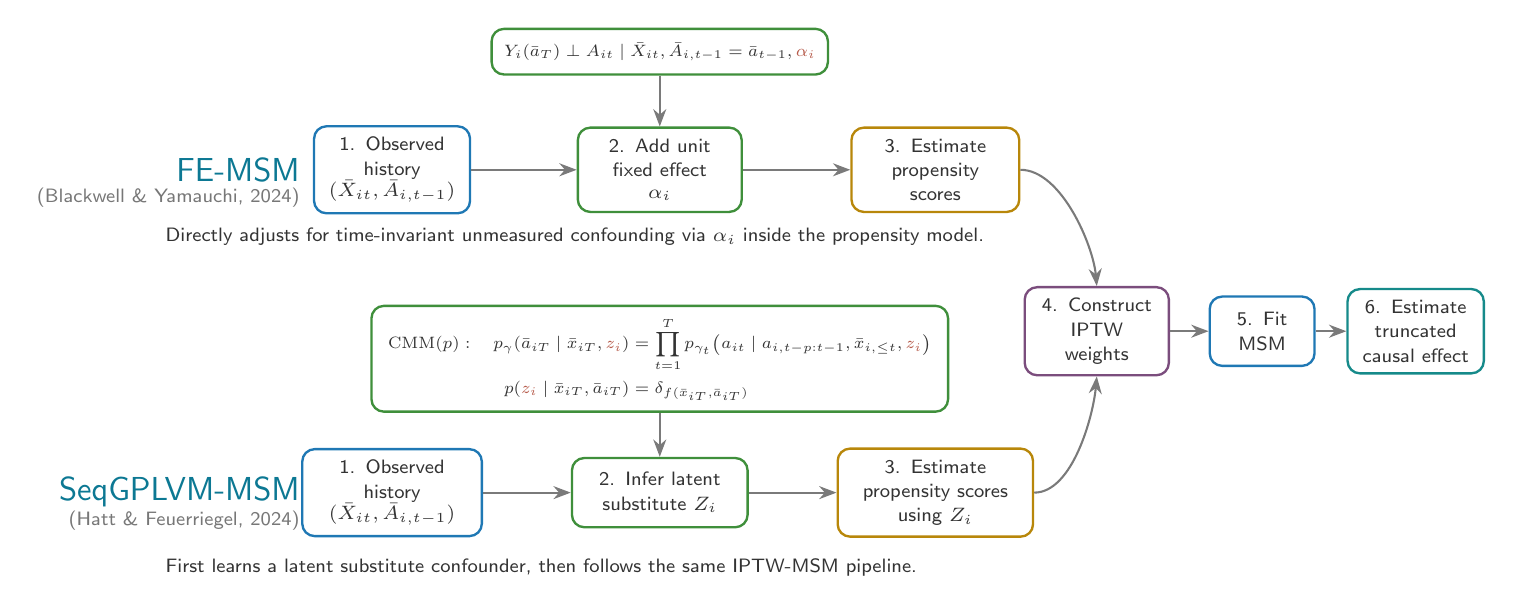
\begin{tikzpicture}[
  x=1cm,y=1cm,
  flow/.style={
    -{Stealth[length=2.2mm]},
    line width=0.75pt,
    draw=PrimerText!65
  },
  stepblue/.style={
    rounded corners=4.5pt,
    line width=0.85pt,
    draw=PipeBlue,
    fill=white,
    align=center,
    minimum height=0.88cm,
    inner sep=4pt,
    font=\fontsize{7.4}{8.8}\selectfont,
    text=PrimerText
  },
  stepgreen/.style={
    rounded corners=4.5pt,
    line width=0.85pt,
    draw=PipeGreen,
    fill=white,
    align=center,
    minimum height=0.88cm,
    inner sep=4pt,
    font=\fontsize{7.4}{8.8}\selectfont,
    text=PrimerText
  },
  stepgold/.style={
    rounded corners=4.5pt,
    line width=0.85pt,
    draw=PipeGold,
    fill=white,
    align=center,
    minimum height=0.88cm,
    inner sep=4pt,
    font=\fontsize{7.4}{8.8}\selectfont,
    text=PrimerText
  },
  steppurple/.style={
    rounded corners=4.5pt,
    line width=0.85pt,
    draw=PipePurple,
    fill=white,
    align=center,
    minimum height=0.92cm,
    inner sep=4pt,
    font=\fontsize{7.4}{8.8}\selectfont,
    text=PrimerText
  },
  stepteal/.style={
    rounded corners=4.5pt,
    line width=0.85pt,
    draw=PipeTeal,
    fill=white,
    align=center,
    minimum height=0.92cm,
    inner sep=4pt,
    font=\fontsize{7.4}{8.8}\selectfont,
    text=PrimerText
  },
  formula/.style={
    rounded corners=4.5pt,
    line width=0.85pt,
    draw=PipeGold,
    fill=white,
    align=center,
    inner sep=4.5pt,
    font=\fontsize{6.7}{8.0}\selectfont,
    text=PrimerText
  },
  methodlabel/.style={
  anchor=east,
  font=\fontsize{12.3}{14.5}\selectfont,
  text=PrimerTeal
  },
  sidenote/.style={
    anchor=west,
    font=\fontsize{7.4}{9.0}\selectfont,
    text=PrimerText,
    align=left
  },
  methodcite/.style={
  anchor=east,
  font=\fontsize{6.8}{8.0}\selectfont,
  text=PrimerMuted
  }
]

% -------------------------------------------------
% Top formula boxes
% -------------------------------------------------
\node[formula, draw=PipeGreen,minimum height=0.58cm] (feassump) at (6.50,5.20)
{\scalebox{0.85}{$
Y_i(\bar a_T)\perp A_{it}
\mid \bar {X}_{it},\bar A_{i,t-1}=\bar a_{t-1},\red{\alpha_i}
$}};

%\node[formula, minimum height=0.58cm] (femodel) at (10,6.20)
%{\scalebox{0.82}{$
%\operatorname{logit}P(A_{it}=1\mid \bar {X}_{it},\bar A_{i,t-1},\alpha_i)
%=
%\alpha_i+\beta^\top {X}_{it}+\phi A_{i,t-1}
%$}};

% -------------------------------------------------
% FE-MSM row
% -------------------------------------------------
\node[methodlabel] at (2.05,3.70) {FE-MSM};
\node[methodcite] at (2.05,3.35) {(Blackwell \& Yamauchi, 2024)};


\node[stepblue, text width=1.70cm] (fe1) at (3.10,3.70)
  {1. Observed\\history\\[-1pt]
  \((\bar {X}_{it},\bar A_{i,t-1})\)};

\node[stepgreen, text width=1.80cm] (fe2) at (6.50,3.70)
{2. Add unit\\fixed effect\\[-1pt]
\(\alpha_i\)};

\node[stepgold, text width=1.85cm] (fe3) at (10,3.70)
{3. Estimate\\propensity\\scores};

\draw[flow] (fe1.east) -- (fe2.west);
\draw[flow] (fe2.east) -- (fe3.west);
%\draw[flow] (fe3.north)--(femodel.south);
\draw[flow] (feassump.south)--(fe2.north);

\node[sidenote] at (0.10,2.85)
{Directly adjusts for time-invariant unmeasured confounding via \(\alpha_i\) inside the propensity model.};

% -------------------------------------------------
% CMM box
% -------------------------------------------------
\node[
  stepgreen,
  minimum width=6.90cm,
  minimum height=0.82cm,
  inner xsep=6pt,
  inner ysep=4pt
] (cmm) at (6.50,1.30)
{\scalebox{.85}{$
\begin{aligned}
\mathrm{CMM}(p):\quad
p_{\gamma}(\bar a_{iT}\mid \bar x_{iT},\red{z_i})
&=
\prod_{t=1}^{T}
p_{\gamma_t}\!\left(
a_{it}\mid a_{i,t-p:t-1},\bar x_{i,\le t},\red{z_i}
\right)
\\[-1pt]
p(\red{z_i}\mid \bar x_{iT},\bar a_{iT})
&=
\delta_{f(\bar x_{iT},\bar a_{iT})}
\end{aligned}
$}};

% -------------------------------------------------
% SeqGPLVM-MSM row
% -------------------------------------------------
\node[methodlabel] at (2.05,-0.40) {SeqGPLVM-MSM};
\node[methodcite] at (2.05,-0.75) {(Hatt \& Feuerriegel, 2024)};

\node[stepblue, text width=2.00cm] (seq1) at (3.10,-0.40)
{1. Observed\\history\\[-1pt]
\((\bar {X}_{it},\bar A_{i,t-1})\)};

\node[stepgreen, text width=1.95cm] (seq2) at (6.50,-0.40)
{2. Infer latent\\substitute \(Z_i\)};

\node[stepgold, text width=2.20cm] (seq3) at (10,-0.40)
{3. Estimate\\propensity scores\\using \(Z_i\)};

\draw[flow] (seq1.east) -- (seq2.west);
\draw[flow] (seq2.east) -- (seq3.west);
\draw[flow] (cmm.south) -- (seq2.north);

\node[sidenote] at (0.10,-1.35)
{First learns a latent substitute confounder, then follows the same IPTW-MSM pipeline.};

% -------------------------------------------------
% Shared IPTW-MSM pipeline
% -------------------------------------------------
\node[steppurple, text width=1.55cm] (w) at (12.05,1.65)
{4. Construct\\IPTW weights};

\node[stepblue, text width=1.05cm] (msm) at (14.15,1.65)
{5. Fit\\MSM};

\node[stepteal, text width=1.45cm] (effect) at (16.10,1.65)
{6. Estimate\\truncated\\causal effect};

% FE and Seq paths into shared step
\draw[flow] (fe3.east)  to[out=0,in=95,looseness=0.75] (w.north);
\draw[flow] (seq3.east) to[out=0,in=-95,looseness=0.75] (w.south);

% Shared pipeline
\draw[flow] (w.east) -- (msm.west);
\draw[flow] (msm.east) -- (effect.west);

\end{tikzpicture}%
}
\end{center}

\end{frame}
%%%%%%%%%%%%%%%%%%%%%%%%%%%%%%%%%%%%%%%%%%%%%%%%%%%
\begin{comment}
% Speaker note: 55 seconds. Contrast the two methods without getting lost in detail: fixed effect versus latent variable inferred from the treatment trajectory.
\begin{frame}{Two methods, one IPTW-MSM pipeline}
\begin{columns}[T,onlytextwidth]
\begin{column}{0.46\textwidth}
{\fontsize{11.0}{14}\selectfont\teal{FE-MSM}}\par
\vspace{0.18cm}

\includegraphics[width=0.74\linewidth]{fixed_effect_dag.pdf}
\vspace{0.08cm}
\spacedparagraph{Use a unit fixed effect \(\alpha_i\) directly in the propensity model.}
\[
\eta_i=\alpha_i
\]
\end{column}
\begin{column}{0.50\textwidth}
{\fontsize{11.0}{14}\selectfont\teal{SeqGPLVM-MSM}}\par
\vspace{0.18cm}

\includegraphics[width=0.92\linewidth]{fit_seqgplvm_dag.pdf}
\vspace{-0.05cm}
\spacedparagraph{Infer a latent variable \(Z_i\) from the treatment trajectory and covariates.}
\[
\eta_i=Z_i
\]
\end{column}
\end{columns}
\vspace{0.10cm}
{\fontsize{9.7}{12.5}\selectfont\RaggedRight Both methods 
then estimate propensity scores, construct IPTW weights, 
and fit the same truncated marginal structural model.\par}
\end{frame}
\end{comment}
% Speaker note: 50 seconds. Explain why the simulation is fair: known DGP, true effects known, same MSM, same target. Stress this uses the final thesis design, not the older draft results.


\begin{frame}{Simulation design: known DGP, known causal effects}

\begin{columns}[T,onlytextwidth]

% ---------------- LEFT COLUMN ----------------
\begin{column}{0.62\textwidth}
\vspace{-0.15cm}

\centering

\includegraphics[width=0.88\linewidth]{dgp_dag.pdf}

\vspace{-0.45cm}

{\fontsize{8.4}{10.8}\selectfont
\begin{align*}
&A_{it}
=
\mathbbm{1}\!\left\{
\eta_{it}
\leq
\operatorname{expit}
\!\left(
\red{U_i}+\phi A_{i,t-1}+\beta^\top X_{it}
\right)
\right\}, \\[0.25em]
&Y_i
=
\red{U_i}+\tau_F A_{iT}
+\tau_C\sum_{t=T-3}^{T-1}A_{it}
+\theta^\top\bar X_i+\epsilon_i,\\[0.25em]
&E[Y_i(\underline{a}_{T-k})]
=
\alpha
+
\tau_F a_T
+
\tau_C
\sum_{t=T-3}^{T-1} a_t .
\end{align*}
}

\vspace{-0.65cm}

{\fontsize{8.2}{10.5}\selectfont

}

\end{column}

% ---------------- RIGHT COLUMN ----------------
\begin{column}{0.35\textwidth}
\vspace{0.95cm}

{\fontsize{9.2}{12.5}\selectfont
\raggedright

\textbf{Design grid}

\vspace{0.15cm}
\noindent\hspace*{0.45cm}%
$\begin{aligned}[t]
&N \in \{200,500,1000\}\\
&\rho = N/T \in \{5,10,50\}\\
&U_i \in [-a,a],
\qquad
a\in\{1,2\}
\end{aligned}$

\vspace{0.65cm}

\textbf{True targets}

\vspace{0.15cm}
\noindent\hspace*{0.45cm}%
$\begin{aligned}[t]
&\tau_F = 1,
\qquad
\tau_C = 0.3
\end{aligned}$
}

\end{column}
\end{columns}
\end{frame}
%%%%%%%%%%%%%%%%%%%%%%%%%%%%%%%%%%%%%%%%%%%%%%%%%%%%%%%%%%%%

% Speaker note: 65 seconds. This is the most important slide. Summarize results accurately from the thesis: both methods help versus naive IPTW, FE-MSM usually better, SeqGPLVM weak with short T/strong U, coverage mixed.
\begin{frame}{Results: adjustment helps, but finite samples matter}
\vspace{-0.25cm}

\begin{columns}[T,onlytextwidth]

% ---------------- LEFT: FIGURE ----------------
\begin{column}{0.67\textwidth}
\vspace{-0.05cm}
\begin{center}

\includegraphics[width=1.02\linewidth]{simulation_bias_a2_p4.pdf}
\end{center}
\end{column}

% ---------------- RIGHT: INTERPRETATION ----------------
\begin{column}{0.30\textwidth}
\vspace{0.55cm}

{\fontsize{8.4}{10.9}\selectfont

\spacedparagraph{
\pstrong{Naive IPTW remains biased} when \(U_i\) is ignored.
}

\spacedparagraph{
Both adjusted methods \teal{move bias closer to zero}, especially as \(N\) increases.
}

\spacedparagraph{
FE-MSM performs best in this DGP, with \teal{lower bias} across most settings.
}

\spacedparagraph{
SeqGPLVM-MSM is most fragile for \(\rho=50\), especially under stronger unmeasured confounding.
}

}

\end{column}

\end{columns}

\vfill
%\smallref{Shown: bias only, two-covariate case with stronger unmeasured confounding, \(a=2\); 500 simulation runs. Coverage results are reported in the backup slides.}

\end{frame}

% Speaker note: 55 seconds. End with a balanced conclusion: the thesis is not just a benchmark, it clarifies assumptions and shows what is needed before practical use.
\begin{frame}{Conclusion: what the comparison shows}
\begin{columns}[T,onlytextwidth]
\begin{column}{0.48\textwidth}
{\fontsize{11}{14}\selectfont\teal{Main contributions}}\par
\vspace{0.25cm}
\spacedparagraph{Unified notation and assumptions for FE-MSM and SeqGPLVM-MSM.}
\spacedparagraph{A detailed derivation of the SeqGPLVM loss function and a modular GPyTorch implementation.}
\spacedparagraph{A simulation comparison under a common causal target and DGP.}
\end{column}
\begin{column}{0.48\textwidth}
{\fontsize{11}{14}\selectfont\teal{Main takeaway}}\par
\vspace{0.25cm}
\spacedparagraph{Both methods replace the usual no-unmeasured-confounding assumption with structural assumptions about a time-invariant hidden factor.}
\spacedparagraph{FE-MSM is simpler and more stable here, but depends on correct propensity specification and within-unit switching.}
\spacedparagraph{SeqGPLVM is more flexible, but relies on strong latent-identifiability assumptions and enough treatment history.}
\end{column}
\end{columns}
\vspace{0.25cm}
{\fontsize{10.3}{14}\selectfont\RaggedRight\red{Bottom line:} promising tools in controlled settings, but not yet general-purpose deconfounding methods.\par}
\end{frame}

\begin{frame}{Future research: interpreting the latent structure}

\vspace{0.15cm}

{\fontsize{11}{15}\selectfont
\spacedparagraph{
Despite their different modeling strategies, FE-MSM and SeqGPLVM-MSM show similar performance for larger \(N\) and \(T\), suggesting a possible link between fixed effects and learned latent variables.
}
\vspace{0.20cm}
\spacedparagraph{
A useful direction for future work is to study whether the latent variables inferred by SeqGPLVM-MSM can be interpreted through the more transparent fixed effects in FE-MSM, helping to better explain and diagnose the latent-variable approach.
}
}

\end{frame}

\begin{frame}{References}

\vspace{-0.05cm}

{\fontsize{10.8}{13.5}\selectfont\teal{Key methodological references}}\par

\vspace{0.30cm}

{\fontsize{8.15}{10.6}\selectfont
\RaggedRight

\noindent
\textcolor{PrimerTeal}{Blackwell \& Yamauchi (2024)}\par
\muted{The effect of political advertising after Citizens United: Adjusting for unmeasured confounding in marginal structural models.}

\vspace{0.22cm}
\textcolor{PrimerRule}{\rule{\linewidth}{0.35pt}}

\vspace{0.22cm}
\noindent
\textcolor{PrimerTeal}{Hatt \& Feuerriegel (2024)}\par
\muted{Sequential deconfounding for causal inference with unobserved confounders. 
Proceedings of the Third Conference on Causal Learning and Reasoning, PMLR, 934--956.}

\vspace{0.22cm}
\textcolor{PrimerRule}{\rule{\linewidth}{0.35pt}}

\vspace{0.22cm}
\noindent
\textcolor{PrimerTeal}{Robins (2000)}\par
\muted{Marginal structural models versus structural nested models as tools for causal inference. 
In \textit{Statistical Models in Epidemiology, the Environment, and Clinical Trials}, 95--133. Springer.}

}

\vfill

{\fontsize{6.4}{8.0}\selectfont
\muted{Main references only; full bibliography in the thesis.}
}

\end{frame}

% ---------------------------------------------------------
% APPENDIX SLIDE 1: SeqGPLVM
% ---------------------------------------------------------
\begin{frame}{Appendix: SeqGPLVM graphical model and estimation idea}
\vspace{-0.35cm}

\begin{columns}[T,onlytextwidth]

% ---------------- LEFT: GRAPHICAL REPRESENTATION ----------------
\begin{column}{0.50\textwidth}
\vspace{0.05cm}

\begin{center}

\includegraphics[width=\linewidth]{fit_seqgplvm_dag.pdf}
\end{center}

\vspace{-0.15cm}
{\fontsize{6.2}{7.5}\selectfont\muted{
Graphical representation of the SeqGPLVM treatment model: \(Z_i\) is inferred from the observed sequence and then used as a substitute confounder.
}}

\end{column}

% ---------------- RIGHT: MATH AND EXPLANATION ----------------
\begin{column}{0.47\textwidth}
\vspace{-0.05cm}

{\fontsize{8.0}{9.6}\selectfont
\pstrong{1. Conditional Markov treatment model}

\vspace{-0.45cm}
\[
p_{\gamma}(\bar a_{iT}\mid \bar x_{iT},\red{z_i})
=
\prod_{t=1}^{T}
p_{\gamma_t}\!\left(
a_{it}\mid a_{i,t-p:t-1},
\bar x_{i,\le t},
\red{z_i}
\right).
\]

\vspace{-0.22cm}
\spacedparagraph{
The latent variable \(Z_i\) is time-invariant and is meant to absorb the stable unmeasured factor that induces dependence across treatments.
}

\vspace{0.05cm}
\pstrong{2. Flexible GP treatment likelihood}

\vspace{-0.45cm}
\[
f_t:
\left(
\red{Z_i},\bar X_{i,\le t},A_{i,t-p:t-1}
\right)
\longrightarrow A_{it},
\qquad
f_t\sim\mathcal{GP}(0,k_t).
\]

\vspace{-0.22cm}
\spacedparagraph{
The GP makes the treatment assignment model non-parametric, so interactions between \(Z_i\), covariates, and past treatments do not need to be fixed in advance.
}

\vspace{0.05cm}
\pstrong{3. Downstream IPTW-MSM}

\vspace{-0.45cm}
\[
z_i^{(s)}\sim q_\psi(Z_i),\qquad
\pi_{it}^{(s)}
=
P(A_{it}=1\mid \bar X_{it},\bar A_{i,t-1},z_i^{(s)}).
\]

\vspace{-0.45cm}
%\[
%\hat\theta
%=
%\frac{1}{S}\sum_{s=1}^{S}\hat\theta^{(s)}.
%\]

\vspace{-0.25cm}
}

\end{column}

\end{columns}

%\smallref{Appendix detail: SeqGPLVM learns a substitute confounder from the treatment process, then uses posterior draws of \(Z_i\) in the same IPTW-MSM pipeline.}

\end{frame}

% ---------------------------------------------------------
% APPENDIX SLIDE 2: FE-MSM ESTIMATION
% ---------------------------------------------------------
\begin{frame}{Appendix: FE-MSM graphical model and estimation}
\vspace{-0.35cm}

\begin{columns}[T,onlytextwidth]

% ---------------- LEFT: GRAPHICAL REPRESENTATION ----------------
\begin{column}{0.47\textwidth}
\vspace{0.05cm}

\begin{center}

\includegraphics[width=\linewidth]{fixed_effect_dag.pdf}
\end{center}

\vspace{-0.10cm}
{\fontsize{6.2}{7.5}\selectfont\muted{
Plate-style representation of the fixed-effect propensity-score model.
}}

\end{column}

% ---------------- RIGHT: ESTIMATION STEPS ----------------
\begin{column}{0.50\textwidth}
\vspace{-0.05cm}

{\fontsize{8.0}{9.6}\selectfont

\pstrong{1. Estimate the treatment assignment model}

\vspace{-0.18cm}
\[
\pi_{it}(\beta,\alpha_i)
=
P(A_{it}=1\mid \bar X_{it},\bar A_{i,t-1},\alpha_i).
\]

\vspace{-0.18cm}
\[
\ell_{it}(\beta,\alpha_i)
=
A_{it}\log \pi_{it}
+
(1-A_{it})\log(1-\pi_{it}).
\]

\vspace{-0.18cm}
\[
(\hat\beta,\hat\alpha_1,\ldots,\hat\alpha_N)
=
\arg\max_{\beta,\alpha_1,\ldots,\alpha_N}
\sum_{i=1}^{N}\sum_{t=1}^{T}
\ell_{it}(\beta,\alpha_i).
\]

\vspace{-0.10cm}
\spacedparagraph{
In practice, this is a fixed-effect binary treatment model, usually implemented as a logistic model with unit-specific intercepts.
}

\vspace{0.05cm}
\pstrong{2. Construct IPTW weights for the last \(k\) periods}

\vspace{-0.20cm}
\[
\widehat W_i
=
\prod_{t=T-k+1}^{T}
\left(\frac{1}{\hat\pi_{it}}\right)^{A_{it}}
\left(\frac{1}{1-\hat\pi_{it}}\right)^{1-A_{it}}.
\]

\vspace{0.05cm}
\pstrong{3. Fit the marginal structural model}

\vspace{-0.18cm}
\[
E[Y_i(\underline{a}_{T-k})]=m(\underline{a}_{T-k};\theta),
\]

\vspace{-0.18cm}
\[
\Psi_N(\theta)
=
\frac{1}{N}\sum_{i=1}^{N}
\widehat W_i
h(A_{i,T-k})
\left[
Y_i-m(A_{i,T-k};\theta)
\right]
=0.
\]

\vspace{-0.25cm}
\arrowtext{For a linear MSM, this last step reduces to a weighted least squares regression of \(Y_i\) on the truncated treatment history.}

}

\end{column}

\end{columns}

\smallref{Appendix detail: FE-MSM controls for time-invariant unmeasured confounding by putting \(\alpha_i\) in the propensity model, then using the resulting weights in the MSM.}

\end{frame}

% ---------------------------------------------------------
% APPENDIX SLIDE: COVERAGE RESULTS
% ---------------------------------------------------------
\begin{frame}{Appendix: coverage under stronger hidden confounding}
\vspace{-0.32cm}

\begin{columns}[T,onlytextwidth]

% ---------------- LEFT: COVERAGE FIGURE ----------------
\begin{column}{0.68\textwidth}
\vspace{-0.05cm}

\begin{center}

\includegraphics[width=1.03\linewidth]{simulation_coverage_a2_p4.pdf}
\end{center}

\vspace{-0.35cm}
{\fontsize{5.9}{7.0}\selectfont
\muted{
Coverage of 90\% confidence intervals over 500 simulation runs. 
Here \(a=2\) corresponds to stronger time-invariant unmeasured confounding.
}
}

\end{column}

% ---------------- RIGHT: INTERPRETATION ----------------
\begin{column}{0.29\textwidth}
\vspace{0.35cm}

{\fontsize{8.0}{9.8}\selectfont

\vspace{-0.35cm}
\spacedparagraph{
The dashed horizontal line is the target: intervals should contain the true effect in about \(90\%\) of repeated samples.
}

\vspace{0.05cm}
\pstrong{Main pattern}

\spacedparagraph{
Naive IPTW has severe \red{undercoverage}, especially for \(\tau_C=0.3\), because it ignores the stable unmeasured confounder \(U_i\).
}

\spacedparagraph{
FE-MSM is usually \teal{closest to IPTW-True}, but still falls below nominal coverage in the harder cumulative-effect panels.
}

%\spacedparagraph{
%SeqGPLVM-MSM is most fragile when \(\rho=50\), i.e. when the treatment history is shortest. Wider uncertainty is not enough to compensate for remaining bias.
%}

\vspace{0.05cm}
\pstrong{Interpretation}

\spacedparagraph{
Coverage confirms the bias result: adjustment helps, but finite-sample uncertainty is still difficult under strong hidden confounding.
}

}

\end{column}

\end{columns}

\vfill
\smallref{Shown: four-covariate case, \(a=2\), \(N\in\{200,500,1000\}\), \(\rho=N/T\in\{5,10,50\}\). Larger \(\rho\) means a shorter treatment sequence.}

\end{frame}
\end{document}
